% Options for packages loaded elsewhere
\PassOptionsToPackage{unicode}{hyperref}
\PassOptionsToPackage{hyphens}{url}
\PassOptionsToPackage{dvipsnames,svgnames,x11names}{xcolor}
%
\documentclass[
  letterpaper,
  DIV=11,
  numbers=noendperiod]{scrartcl}

\usepackage{amsmath,amssymb}
\usepackage{iftex}
\ifPDFTeX
  \usepackage[T1]{fontenc}
  \usepackage[utf8]{inputenc}
  \usepackage{textcomp} % provide euro and other symbols
\else % if luatex or xetex
  \usepackage{unicode-math}
  \defaultfontfeatures{Scale=MatchLowercase}
  \defaultfontfeatures[\rmfamily]{Ligatures=TeX,Scale=1}
\fi
\usepackage{lmodern}
\ifPDFTeX\else  
    % xetex/luatex font selection
\fi
% Use upquote if available, for straight quotes in verbatim environments
\IfFileExists{upquote.sty}{\usepackage{upquote}}{}
\IfFileExists{microtype.sty}{% use microtype if available
  \usepackage[]{microtype}
  \UseMicrotypeSet[protrusion]{basicmath} % disable protrusion for tt fonts
}{}
\makeatletter
\@ifundefined{KOMAClassName}{% if non-KOMA class
  \IfFileExists{parskip.sty}{%
    \usepackage{parskip}
  }{% else
    \setlength{\parindent}{0pt}
    \setlength{\parskip}{6pt plus 2pt minus 1pt}}
}{% if KOMA class
  \KOMAoptions{parskip=half}}
\makeatother
\usepackage{xcolor}
\setlength{\emergencystretch}{3em} % prevent overfull lines
\setcounter{secnumdepth}{-\maxdimen} % remove section numbering
% Make \paragraph and \subparagraph free-standing
\ifx\paragraph\undefined\else
  \let\oldparagraph\paragraph
  \renewcommand{\paragraph}[1]{\oldparagraph{#1}\mbox{}}
\fi
\ifx\subparagraph\undefined\else
  \let\oldsubparagraph\subparagraph
  \renewcommand{\subparagraph}[1]{\oldsubparagraph{#1}\mbox{}}
\fi


\providecommand{\tightlist}{%
  \setlength{\itemsep}{0pt}\setlength{\parskip}{0pt}}\usepackage{longtable,booktabs,array}
\usepackage{calc} % for calculating minipage widths
% Correct order of tables after \paragraph or \subparagraph
\usepackage{etoolbox}
\makeatletter
\patchcmd\longtable{\par}{\if@noskipsec\mbox{}\fi\par}{}{}
\makeatother
% Allow footnotes in longtable head/foot
\IfFileExists{footnotehyper.sty}{\usepackage{footnotehyper}}{\usepackage{footnote}}
\makesavenoteenv{longtable}
\usepackage{graphicx}
\makeatletter
\def\maxwidth{\ifdim\Gin@nat@width>\linewidth\linewidth\else\Gin@nat@width\fi}
\def\maxheight{\ifdim\Gin@nat@height>\textheight\textheight\else\Gin@nat@height\fi}
\makeatother
% Scale images if necessary, so that they will not overflow the page
% margins by default, and it is still possible to overwrite the defaults
% using explicit options in \includegraphics[width, height, ...]{}
\setkeys{Gin}{width=\maxwidth,height=\maxheight,keepaspectratio}
% Set default figure placement to htbp
\makeatletter
\def\fps@figure{htbp}
\makeatother

\KOMAoption{captions}{tableheading}
\makeatletter
\@ifpackageloaded{tcolorbox}{}{\usepackage[skins,breakable]{tcolorbox}}
\@ifpackageloaded{fontawesome5}{}{\usepackage{fontawesome5}}
\definecolor{quarto-callout-color}{HTML}{909090}
\definecolor{quarto-callout-note-color}{HTML}{0758E5}
\definecolor{quarto-callout-important-color}{HTML}{CC1914}
\definecolor{quarto-callout-warning-color}{HTML}{EB9113}
\definecolor{quarto-callout-tip-color}{HTML}{00A047}
\definecolor{quarto-callout-caution-color}{HTML}{FC5300}
\definecolor{quarto-callout-color-frame}{HTML}{acacac}
\definecolor{quarto-callout-note-color-frame}{HTML}{4582ec}
\definecolor{quarto-callout-important-color-frame}{HTML}{d9534f}
\definecolor{quarto-callout-warning-color-frame}{HTML}{f0ad4e}
\definecolor{quarto-callout-tip-color-frame}{HTML}{02b875}
\definecolor{quarto-callout-caution-color-frame}{HTML}{fd7e14}
\makeatother
\makeatletter
\makeatother
\makeatletter
\makeatother
\makeatletter
\@ifpackageloaded{caption}{}{\usepackage{caption}}
\AtBeginDocument{%
\ifdefined\contentsname
  \renewcommand*\contentsname{Table of contents}
\else
  \newcommand\contentsname{Table of contents}
\fi
\ifdefined\listfigurename
  \renewcommand*\listfigurename{List of Figures}
\else
  \newcommand\listfigurename{List of Figures}
\fi
\ifdefined\listtablename
  \renewcommand*\listtablename{List of Tables}
\else
  \newcommand\listtablename{List of Tables}
\fi
\ifdefined\figurename
  \renewcommand*\figurename{Figure}
\else
  \newcommand\figurename{Figure}
\fi
\ifdefined\tablename
  \renewcommand*\tablename{Table}
\else
  \newcommand\tablename{Table}
\fi
}
\@ifpackageloaded{float}{}{\usepackage{float}}
\floatstyle{ruled}
\@ifundefined{c@chapter}{\newfloat{codelisting}{h}{lop}}{\newfloat{codelisting}{h}{lop}[chapter]}
\floatname{codelisting}{Listing}
\newcommand*\listoflistings{\listof{codelisting}{List of Listings}}
\makeatother
\makeatletter
\@ifpackageloaded{caption}{}{\usepackage{caption}}
\@ifpackageloaded{subcaption}{}{\usepackage{subcaption}}
\makeatother
\makeatletter
\@ifpackageloaded{tcolorbox}{}{\usepackage[skins,breakable]{tcolorbox}}
\makeatother
\makeatletter
\@ifundefined{shadecolor}{\definecolor{shadecolor}{rgb}{.97, .97, .97}}
\makeatother
\makeatletter
\makeatother
\makeatletter
\makeatother
\makeatletter
\@ifpackageloaded{fontawesome5}{}{\usepackage{fontawesome5}}
\makeatother
\ifLuaTeX
  \usepackage{selnolig}  % disable illegal ligatures
\fi
\IfFileExists{bookmark.sty}{\usepackage{bookmark}}{\usepackage{hyperref}}
\IfFileExists{xurl.sty}{\usepackage{xurl}}{} % add URL line breaks if available
\urlstyle{same} % disable monospaced font for URLs
\hypersetup{
  pdftitle={Buridan's ass},
  pdfauthor={Felix Schönbrodt},
  colorlinks=true,
  linkcolor={blue},
  filecolor={Maroon},
  citecolor={Blue},
  urlcolor={Blue},
  pdfcreator={LaTeX via pandoc}}

\title{Buridan's ass}
\usepackage{etoolbox}
\makeatletter
\providecommand{\subtitle}[1]{% add subtitle to \maketitle
  \apptocmd{\@title}{\par {\large #1 \par}}{}{}
}
\makeatother
\subtitle{Your first modeling challenge}
\author{Felix Schönbrodt}
\date{2023-10-20}

\begin{document}
\maketitle
\ifdefined\Shaded\renewenvironment{Shaded}{\begin{tcolorbox}[borderline west={3pt}{0pt}{shadecolor}, boxrule=0pt, frame hidden, sharp corners, interior hidden, enhanced, breakable]}{\end{tcolorbox}}\fi

\hypertarget{buridans-ass}{%
\section{Buridan's Ass}\label{buridans-ass}}

\begin{figure}

{\centering 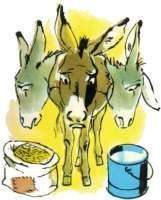
\includegraphics[width=\textwidth,height=4.16667in]{img/Buridans_ass.jpeg}

}

\end{figure}

\begin{quote}
„The man who is violently, but equally, hungry and thirsty, and stands
at an equal distance from food and drink, and who therefore must remain
where he is.``

Aristoteles: \emph{De Caelo/On the Heavens}. Trans. W. K. C. Guthrie,
Heinemann, London 1938, 2:13:295b (S. 237)
\end{quote}

https://p8.storage.canalblog.com/87/85/553105/80715840.jpeg

See \href{https://de.wikipedia.org/wiki/Buridans_Esel}{Wikipedia}

\hypertarget{the-demiurg}{%
\subsection{The demiurg}\label{the-demiurg}}

\begin{figure}

{\centering 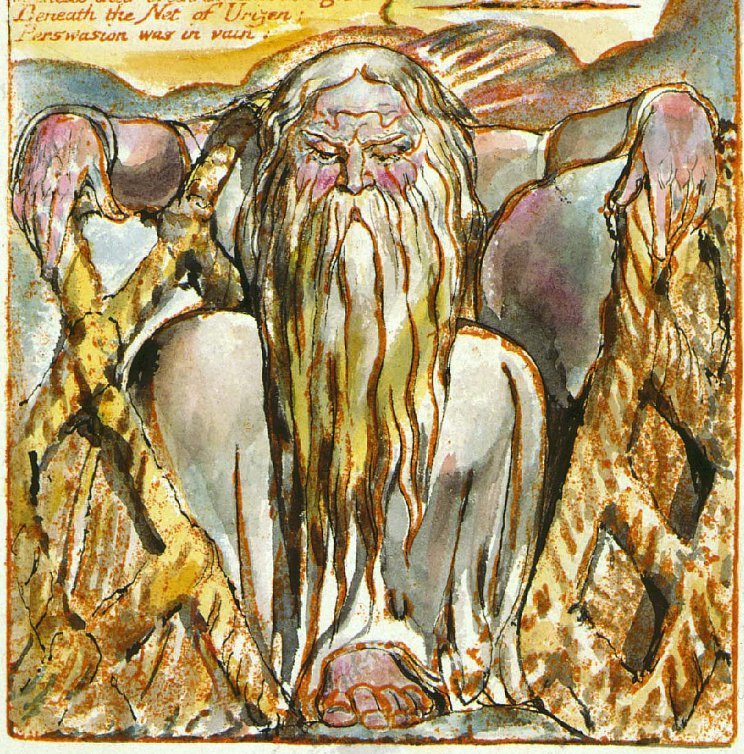
\includegraphics[width=\textwidth,height=4.16667in]{img/Urizen_with_his_net_-_The_Book_of_Urizen,_copy_G,_object_27_c1818_(Library_of_Congress)_Detail.jpg}

}

\end{figure}

\begin{quote}
``Die Gnosis kannte die Gestalt des Demiurgen, eines Schöpfergottes von
niederem Rang, der von der Hochgottheit den Auftrag erhalten hatte, den
Kosmos zu erbauen''

\emph{N. Bischof (in prep, S. 143)}
\end{quote}

\begin{quote}
{\emph{The gnosis knew the figure of the Demiurge, a creator god of
lower rank, who had received the commission from the High Deity to build
the cosmos}}
\end{quote}

By
\href{https://commons.wikimedia.org/w/index.php?curid=28922594}{Dmitrismirnov
- Own work}, CC BY-SA 3.0

\hypertarget{das-demiurgische-prinzip}{%
\subsection{Das demiurgische Prinzip}\label{das-demiurgische-prinzip}}

\begin{quote}
Der Forscher, der eine komplexe Struktur verstehen will, ist gut
beraten, wenn er sich in die Rolle eines solchen Demiurgen versetzt und
sich vorstellt, er hätte sie selbst konstruieren müssen. Natürlich muss
er dafür eine begründete Vermutung haben, was sie leisten soll. Leistung
schließt immer eine Zielvorgabe ein, die Arbeit des Demiurgen läuft also
naturgemäß im Rahmen einer telischen Heuristik \footnote{griechisch
  τέλος (telos): ‚Zweck`, ‚Ziel`, ‚Ende`. Der Zweck ist hier evolutionär
  gedacht: Was hilft dem Überleben und der Fortpflanzung?} ab.

\emph{N. Bischof (in prep, S. 143)}
\end{quote}

{The researcher who wants to understand a complex structure is well
advised to put himself in the role of such a demiurge and imagine that
he would have had to construct it himself. Of course, to do this he must
have an educated guess as to what it should perform. Performance always
includes a target, so the demiurge's work naturally runs within the
framework of a telic heuristic.}

\hypertarget{the-demiurgic-principle}{%
\subsection{The Demiurgic Principle}\label{the-demiurgic-principle}}

\hypertarget{preliminary-version}{%
\subsubsection{Preliminary version}\label{preliminary-version}}

\begin{tcolorbox}[enhanced jigsaw, coltitle=black, opacityback=0, toprule=.15mm, colback=white, colframe=quarto-callout-note-color-frame, bottomtitle=1mm, breakable, leftrule=.75mm, left=2mm, opacitybacktitle=0.6, title=\textcolor{quarto-callout-note-color}{\faInfo}\hspace{0.5em}{Note}, bottomrule=.15mm, toptitle=1mm, titlerule=0mm, colbacktitle=quarto-callout-note-color!10!white, rightrule=.15mm, arc=.35mm]

Wäre ich ein Ingenieur, der einen Mechanismus so konstruieren soll, dass
er eine Leistung des Organismus ebenso gut wie dieser erbringt und dabei
möglichst dieselben Fehler macht -- wie würde ich dann vorgehen? {If I
were an engineer and I had to design a mechanism that performs as well
as the organism and makes the same mistakes -- how would I go about it?}

\end{tcolorbox}

Bischof (in prep, S. 143)

\hypertarget{buridans-ass-level-1-intuitive-modeling}{%
\section{Buridan's ass, level 1: Intuitive
modeling}\label{buridans-ass-level-1-intuitive-modeling}}

\hypertarget{fa-people-group-size1x-group-exercise-cover-your-ass-level-1}{%
\subsection{\texorpdfstring{{\faIcon{people-group} Group exercise: Cover
your ass, Level
1}}{ Group exercise: Cover your ass, Level 1}}\label{fa-people-group-size1x-group-exercise-cover-your-ass-level-1}}

\textbf{Scenario}: The environment has two sources (food and water), in
a substantial distance from each other. The donkey has a general
metabolism that continuously consumes food and water reserves in the
body. As soon as one of the two reserves in the body drops to zero, the
donkey dies.

\textbf{(Simplifying) assumptions}:

\begin{itemize}
\tightlist
\item
  Linear decrease in both water and food reserves in the body, higher
  under activity (e.g., traveling).
\item
  No other needs or tasks (e.g., no predators, no sleep necessary).
\item
  Eating, drinking, and traveling takes a substantial amount of time.
\item
  The donkey has a representation of the environment and knows where the
  two (unlimited) sources are.
\end{itemize}

\textbf{Task}: Construct an organism, with as \emph{few} assumptions as
possible, that survives as long as possible. Which constructs / sensors
/ abilities are necessary for this? Assume as simple abilities as
possible - certainly not super-human abilities. (Rather think of an
amoeba, not a super-AI).

\textbf{Deliverable}: A markdown text file with a verbal description of
the organism. Give it the version number \texttt{0.1.0}.

\begin{figure}

{\centering 
\includegraphics[width=\textwidth,height=0.72917in]{img/buri1.png}

}

\end{figure}

\hypertarget{buridans-ass-level-2-draw-your-diagram}{%
\section{Buridan's ass, level 2: Draw your
diagram}\label{buridans-ass-level-2-draw-your-diagram}}

\hypertarget{the-demiurgic-principle-1}{%
\subsection{The Demiurgic Principle}\label{the-demiurgic-principle-1}}

\hypertarget{final-version}{%
\subsubsection{Final version}\label{final-version}}

\begin{tcolorbox}[enhanced jigsaw, coltitle=black, opacityback=0, toprule=.15mm, colback=white, colframe=quarto-callout-note-color-frame, bottomtitle=1mm, breakable, leftrule=.75mm, left=2mm, opacitybacktitle=0.6, title=\textcolor{quarto-callout-note-color}{\faInfo}\hspace{0.5em}{Note}, bottomrule=.15mm, toptitle=1mm, titlerule=0mm, colbacktitle=quarto-callout-note-color!10!white, rightrule=.15mm, arc=.35mm]

Wäre ich ein Ingenieur, der, \emph{aufbauend auf der letzten
funktionstüchtigen Vorform}, einen Mechanismus so konstruieren soll,
dass er eine Leistung des Organismus ebenso gut wie dieser erbringt und
dabei möglichst dieselben Fehler macht -- wie würde ich dann vorgehen?
{If I were an engineer and, \emph{building upon the last functional
(evolutionary) preform}, I had to design a mechanism that performs as
well as the organism and makes the same mistakes -- how would I go about
it?}

\end{tcolorbox}

{→ Assume realistic capabilities, which respect the evolutionary path
dependency.}

E.g., don't assume \ldots{}

\begin{itemize}
\tightlist
\item
  Mammal organisms that need 3 hands to perform a task
\item
  Omniscient knowledge about the environment, probabilities, distant
  events, the future, \ldots{}
\item
  Unlimited cognitive processing capabilities (``In the first 2ms, the
  simulated amoeba performs a multidimensional Bayesian optimization
  task'')
\end{itemize}

Bischof (in prep, S. 143)

\hypertarget{fa-people-group-size1x-group-exercise-cover-your-ass-level-2}{%
\subsection{\texorpdfstring{{\faIcon{people-group} Group exercise: Cover
your ass, Level
2}}{ Group exercise: Cover your ass, Level 2}}\label{fa-people-group-size1x-group-exercise-cover-your-ass-level-2}}

\hypertarget{draw-a-graphical-model-bischof-style}{%
\subsubsection{Draw a graphical model,
Bischof-style}\label{draw-a-graphical-model-bischof-style}}

Consider the underlying psychological research question: \emph{How can
an organism solve an approach-approach conflict?}

\textbf{Task}: Sketch your initial verbal model in the
\href{../../skills/Bischof-Notation/Bischof-Notation.qmd}{style of
Bischof}. Refine and extend where necessary, e.g.:

\begin{itemize}
\tightlist
\item
  Think about which sensors are necessary (both towards internal states
  and towards the environment) and which actors are necessary
\item
  Give a label to every variable (i.e., every arrow in the graphical
  model).
\end{itemize}

\textbf{Deliverables}:

\begin{itemize}
\tightlist
\item
  Draw the model collaboratively in
  \href{https://www.drawio.com}{draw.io}. In one corner, add the version
  number \texttt{0.2.0} and today's date (simply as a text box).
\item
  Export the model as an \texttt{xml} file and push it to your group's
  Github repo.
\item
  Write a meaningful commit message,
  e.g.~\texttt{Initial\ commit;\ model\ version\ 0.2.0}
\end{itemize}

\begin{figure}

{\centering 
\includegraphics[width=\textwidth,height=0.72917in]{img/buri1.png}

}

\end{figure}

\hypertarget{buridans-ass-level-3}{%
\section{Buridan's ass, level 3}\label{buridans-ass-level-3}}

\hypertarget{fa-people-group-size1x-group-exercise-cover-your-ass-level-3}{%
\subsection{\texorpdfstring{{\faIcon{people-group} Group exercise: Cover
your ass, Level
3}}{ Group exercise: Cover your ass, Level 3}}\label{fa-people-group-size1x-group-exercise-cover-your-ass-level-3}}

\hypertarget{construct-and-variable-definitions}{%
\subsubsection{Construct and variable
definitions}\label{construct-and-variable-definitions}}

In the previous lecture, you learned how a good construct definition
looks like. Apply that new skill to your model!

\textbf{Task}:

\begin{itemize}
\tightlist
\item
  Develop proper definitions for \emph{all} variables and concepts in
  your model
\item
  If necessary, update the model structure in
  \href{https://www.drawio.com}{draw.io}; increase either the
  \emph{minor} version (e.g., to \texttt{0.3.0}) or only the
  \emph{patch} version (e.g., \texttt{0.2.1}); export a new \texttt{xml}
  file.
\item
  Provide the definitions of the model's variables and constructs in a
  separate markdown file (\texttt{Definitions.md}).
\end{itemize}

\textbf{Deliverables}:

\begin{itemize}
\tightlist
\item
  Create a \texttt{CHANGELOG.md} file that explains the changes in the
  model in more detail.
\item
  Push all new files to your group's Github repo.
\item
  Write a meaningful commit message that explains the changes.
\end{itemize}

\begin{figure}

{\centering 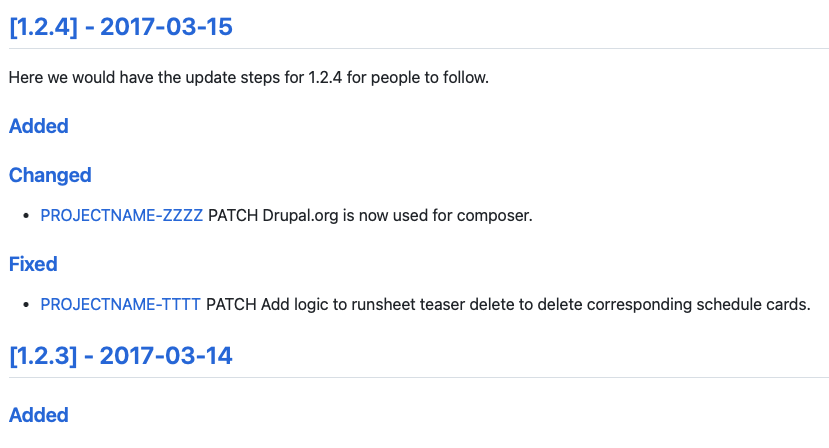
\includegraphics{img/changelog_example.png}

}

\end{figure}

\hypertarget{buridans-ass-level-4}{%
\section{Buridan's ass, level 4}\label{buridans-ass-level-4}}

\hypertarget{fa-people-group-size1x-group-exercise-cover-your-ass-level-4}{%
\subsection{\texorpdfstring{{\faIcon{people-group} Group exercise: Cover
your ass, Level
4}}{ Group exercise: Cover your ass, Level 4}}\label{fa-people-group-size1x-group-exercise-cover-your-ass-level-4}}

\hypertarget{variable-scaling-netlogo-implementation}{%
\subsubsection{Variable Scaling \& Netlogo
Implementation}\label{variable-scaling-netlogo-implementation}}

\textbf{Tasks}:

\begin{itemize}
\tightlist
\item
  Define the \textbf{variables} in the implemented model:

  \begin{itemize}
  \tightlist
  \item
    Scale level
  \item
    Possible range or discrete values (define the set)
  \item
    Interpretability (what does a value of 0.7 mean?)

    \begin{itemize}
    \tightlist
    \item
      Maybe define operationalizations that give a meaning to the
      numbers
    \end{itemize}
  \end{itemize}
\item
  Define computations for each \textbf{box}: How exactly are input
  variables transformed into the output variables? You need a concrete
  formula for that. Theories rarely are so specific that you can
  directly derive a formula; you probably need to fill many gaps with
  ad-hoc assumptions.
\item
  \textbf{Implement} the model in Netlogo
\end{itemize}

\textbf{Deliverables}:

\begin{itemize}
\tightlist
\item
  Push the \texttt{.nlogo} file to your group's Github repo.
\item
  Update all written model descriptions, increase model version.
\item
  Explain \& justify the changes in the model in your
  \texttt{CHANGELOG.md}.
\item
  Write a meaningful commit message.
\end{itemize}

\hypertarget{end}{%
\section{End}\label{end}}

\hypertarget{contact}{%
\subsection{Contact}\label{contact}}

@nicebread@scicomm.xyz

ed.uml.ysp@tdorbneohcs.xilef

https://www.nicebread.de

https://github.com/nicebread

\begin{figure}

{\centering 

\href{http://creativecommons.org/licenses/by-sa/4.0/}{
\includegraphics{Buri_files/mediabag/88x31.png}}

}

\caption{CC-BY-SA 4.0}

\end{figure}



\end{document}
